\subsection{OpenID Connect}

O OpenID Connect (OIDC) é um padrão de camada de identificação em cima do protocolo OAuth 2.0. Utiliza 
todos os conceitos, \emph{tokens} e fluxos do protocolo OAuth 2.0, com a adição do fornecimento de 
atributos do usuário. Esses atributos podem ser 
fornecidos para um sistema por meio de uma API RESTful \texttt{userinfo} ou por meio de um 
\emph{token} de identificação \cite{BIEHL2019}.

O OIDC implementa autenticação como uma extensão da autorização fornecida pelo protocolo OAuth 2.0 
\cite{OIDCCORE}. Similar com o fluxo do OAuth, este método segue as seguintes etapas:

\begin{itemize}
    \item O cliente redireciona para o servidor de autenticação (Provedor OIDC) com os parâmetros 
    necessários (ID do cliente, URI de redirecionamento, etc.);
    \item O provedor apresenta uma página de login ao usuário;
    \item Após login bem sucedido, é solicitada a permissão de acesso aos recursos para o usuário;
    \item O provedor OIDC redireciona o usuário ao cliente, com o código de autorização;
    \item O cliente solicita ao provedor OIDC um \emph{token} de identificação e também geralmente
\emph{tokens} de acesso e atualização;
    \item O provedor envia ao cliente os \emph{tokens} que podem ser utilizados para acessar 
informações do usuário (\emph{endpoint} \texttt{userinfo}), recursos protegidos e solicitar novos 
\emph{tokens} \cite{OIDCCORE}.
\end{itemize}

Um exemplo de funcionamento de uma autenticação utilizando OIDC é mostrado na figura 
\ref{fig:OpenID}

\begin{figure}[ht]
    \centering
    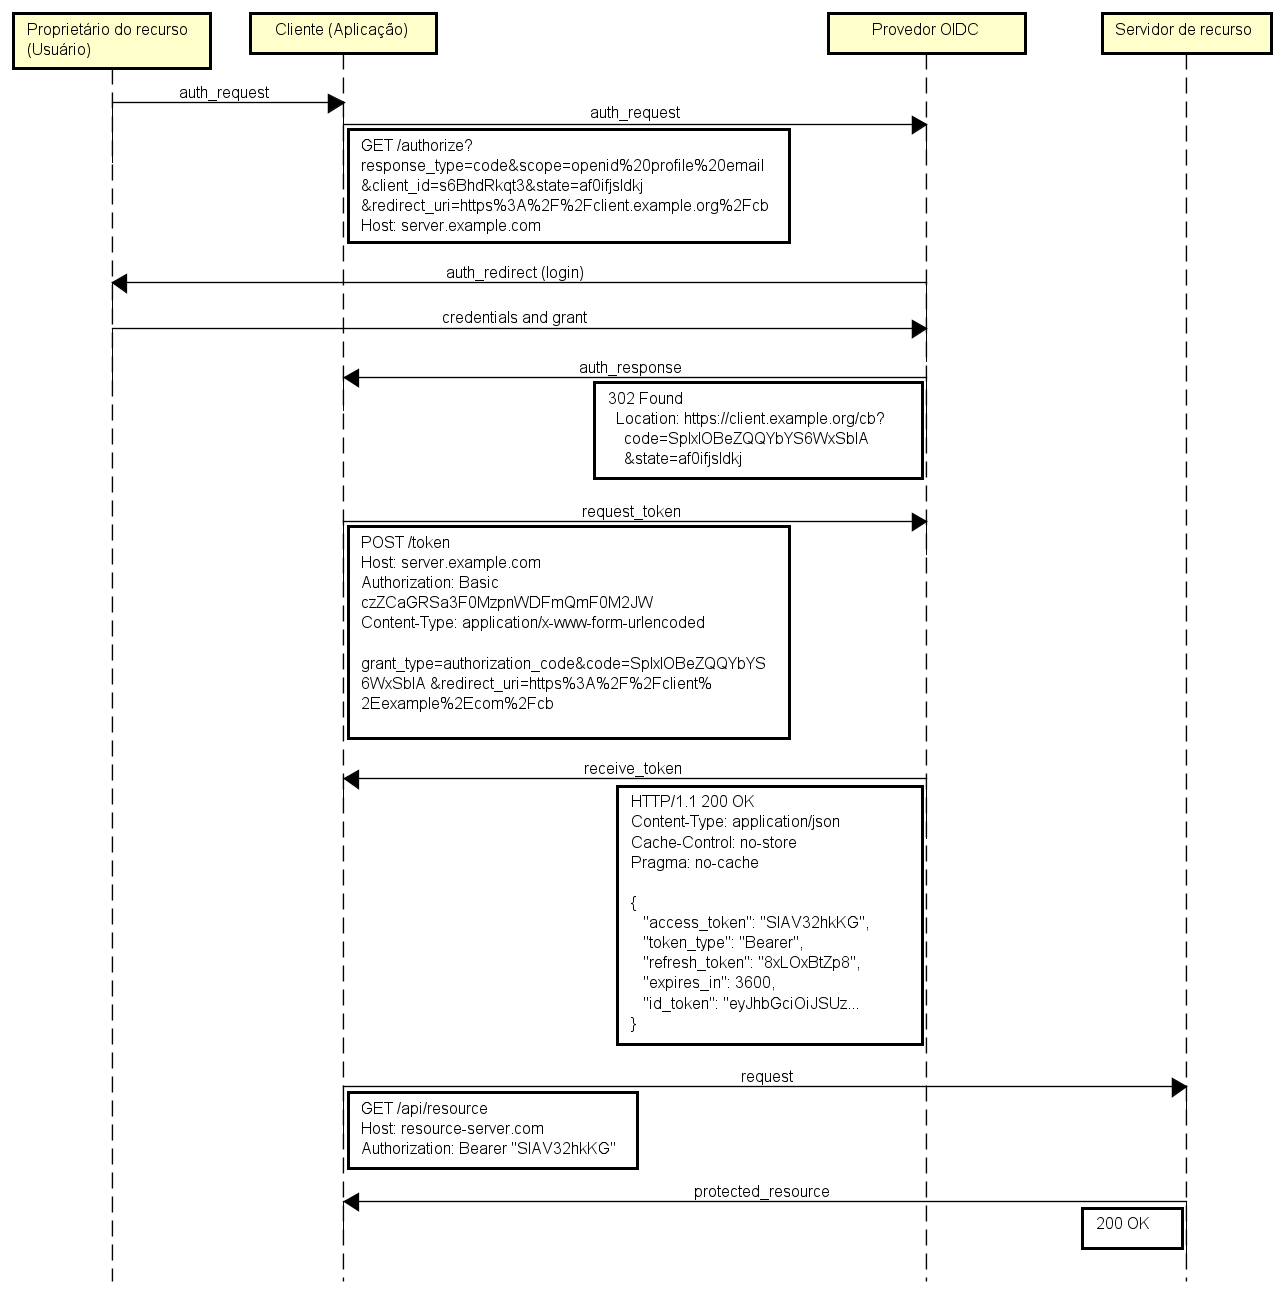
\includegraphics[width=0.95\textwidth]{OpenID Connect.png}
    \caption{Exemplo de autenticação utilizando OpenID Connect}
    \label{fig:OpenID}
\end{figure}